\documentclass[twoside,openright]{uva-bachelor-thesis}

\usepackage[dutch]{babel}  % uncomment if you write in dutch
\usepackage{graphicx}
\usepackage{epstopdf}
\usepackage{url}
\usepackage{algorithmic}
\usepackage{amssymb}
\usepackage{amsmath}
\usepackage[]{algorithm2e}
\usepackage{pifont}

% Title Page
\title{Graphical geography-based \\selection of news items}
\author{Thomas van Ophem}
\supervisors{Raphael 'kena' Poss (UvA)}
\signedby{}


\begin{document}
\maketitle

\begin{abstract}
	Nieuws is normaal gesproken gerepresenteerd rondom een bepaald onderwerp, de lezer haalt de locatie uit de tekst. Zoekmachines zijn onderwerp of keyword gebaseerd; Er is op dit moment geen mogelijkheid om nieuws te zoeken aan de hand van een geografische locatie of een gebied. Dit kan beter, in deze scriptie zal een tool voorgesteld worden om niewus te kunnen zoeken aan de hand van een geslecteerd gebied op een kaart. %uitbreiden
\end{abstract}

\tableofcontents

\chapter{Inleiding}
	\section{Context}
		% iets over het steeds meer en sneller beschikbaar komen van nieuws, niet duidelijk waar het vandaan komt????
		Nieuws is normaal gesproken gerepresenteerd rondom een bepaald onderwerp, de lezer haalt de locatie uit de tekst. Zoekmachines zijn onderwerp of keyword gebaseerd; Er is op dit moment geen mogelijkheid om nieuws te zoeken aan de hand van een geografische locatie of een gebied.
	\section{Bestaande middelen}
		Op dit moment kan er naar nieuws gezocht worden via  nieuws websites zoals bijvoorbeeld Reuters\footnote{http://www.reuters.com/}, Associated Press\footnote{http://www.ap.org/}, NU\footnote{http://www.nu.nl/}. Daarnaast is het mogelijk om nieuws te zoeken via zoekmachines zoals Google News\footnote{https://news.google.nl/} en Bing News\footnote{https://www.bing.com/?scope=news}.
		\\[0.5cm]
		Aan \textit{The University of Maryland} wordt er bij het \textit{computer science department} al 30 jaar onderzoek gedaan naar de zogenaamde \textit{"spatial browsers"}. Dit zijn browsers/zoekmachines waarmee de geografische informatie uit de resultaten inzichtelijker gemaakt wordt voor de gebruiker, maar waarmee ook gezocht kan worden aan de hand van geografische informatie. Het meeste recente systeem wat door het \textit{computer science department} van \textit{The University of Maryland} ontwikkeld is is NewsStand, meer hier over in hoofdstuk \ref{ch:related}.
	\section{Probleem stelling}
		Wie op dit moment naar nieuws wil zoeken doet dit aan de hand van zoektermen gericht op een onderwerp of enkele locatie. Voor het nieuws over een brand in Amsterdam kan gezocht worden met bijvoorbeeld de zoekterm "brand Amsterdam". Dit is voor relatief eenvoudige zoektermen, waar er alleen gekeken wordt naar een stad geen probleem. Maar stel dat je wilt weten wat er op dit moment gaande is in Noord Holland. Welke zoektermen moeten dan gebruikt worden? 
		\\[0.5cm]
		Het probleem wordt nog groter als je gaat kijken naar grotere (internationale) gebieden, stel je wilt weten wat er gaande is rondom de Zwarte Zee. Om hier al het nieuws voor te vinden moet gezocht worden naar het nieuws in alle omliggende landen. Dit resulteerd in een groot aantal zoektermen, met als gevolg dat je veel tijd kwijt bent om een duidelijk beeld te krijgen van wat er in het betreffende gebied gaande is, of dat er helemaal niet gezocht wordt. Gevolg hiervan is dat mensen, burgers, een beperkt/beperkter begrip hebben van het nieuws. Hierdoor krijgen burgers geen of geen goede informatie over wat er gaande is in de wereld, worden zij zich niet bewust van politieke processen met als risico dat zij niet de juiste beslissingen nemen, en belanghebbenden een (mogelijk verkeerde) invloed uit kunnen oefenen.
		\\[0.5cm]
		Een mogelijke oplossing hiervoor is een tool waarmee het mogelijk is om op gebied te zoeken, bijvoorbeeld door een gebied te selecteren op een kaart waar vervolgens het nieuws bijgezocht wordt. Hiermee krijgen burgers een duidelijker beeld van poltieke processen, en zaken die hun leven kunnen be\"invloeden. Daarnaast wordt het mogelijk om de kern en de oorzaken van problemen in de wereld beter te begrijpen.	
	\section{Over dit onderzoek}
		Ik ga een tool ontwikkelen waarbij het mogelijk is om een gebied op een kaart te selecteren waar het nieuws bij gezocht zal worden. In eerste instantie zal ik hierbij gebruik maken van \textit{Bing News} en \textit{Google News}, vervolgens gaat er gebruik gemaakt worden van lokale nieuwsbronnen. Deze nieuwsbronnen hangen dus af van het gekozen gebied. Voor beide implementaties ga ik onderzoeken wat de toegevoegde waarde van de tool is.
		\\[0.5cm]
		De hoofdvraag in dit onderzoek is:
		\\[0.5cm]
		\indent \textit{Wat is de toegevoegde waarde van het zoeken van nieuwsberichten aan de hand van een locatie?}
		\\[0.5cm]
		In deze scriptie zal ik bespreken hoe de tool tot stand is gekomen, welke ontwerp keuzen er zijn gemaakt en hoe deze ge"implementeerd zijn. Daarnaast zal de opzet van het onderzoek en de resultaten besproken worden.
\chapter{Gerelateerd onderzoek}
	\label{ch:related}
	% iest over sinds wanneer umd al onderzoek doet naar dit onderwerp?
	In november 2008 is er het artikel, \textit{NewsStand: A New View on News} \cite{NewsStand2008}, verschenen. Dit onderzoek gaat verder op een artikel geplubliceerd in november 2007, \textit{STEWARD: Architecture of a Spatio-Textual Search Engine} \cite{STEWARD}. Eind 2014 is er van de zelfde groep onderzoekers, verbonden aan \textit{The University of Maryland}, nog een artikel verschenen: \textit{Reading News with maps by Exploiting Spatial Synonyms \cite{RNwMbESS}}. In deze onderzoeken wordt gekeken of het mogelijk is om gebruik te maken van de geografische informatie die (vaak) in nieuwsberichten verwerkt is, en hoe dit dan gebruikt zou kunnen worden. Er wordt hier echter nog niet gekeken naar de mogelijkheid om op een kaart een gebied te selecteren en daar het nieuws bij te zoeken.
	\section{STEWARD: Architecture of a Spatio-Textual Search Engine \cite{STEWARD}}
		STEWARD (\textit{"Spatio-Textual Extraction on the Web Aiding Retrieval of Documents"}) \footnote{http://steward.umiacs.umd.edu/} is een systeem voor het extraheren, opvragen en visualiseren van referenties naar geografische locaties in tekst. In dit artikel wordt besproken hoe het systeem tot stand is gekomen en wat de mogelijkheden van het systeem zijn.
		\begin{figure}[!htb]
			\centering
			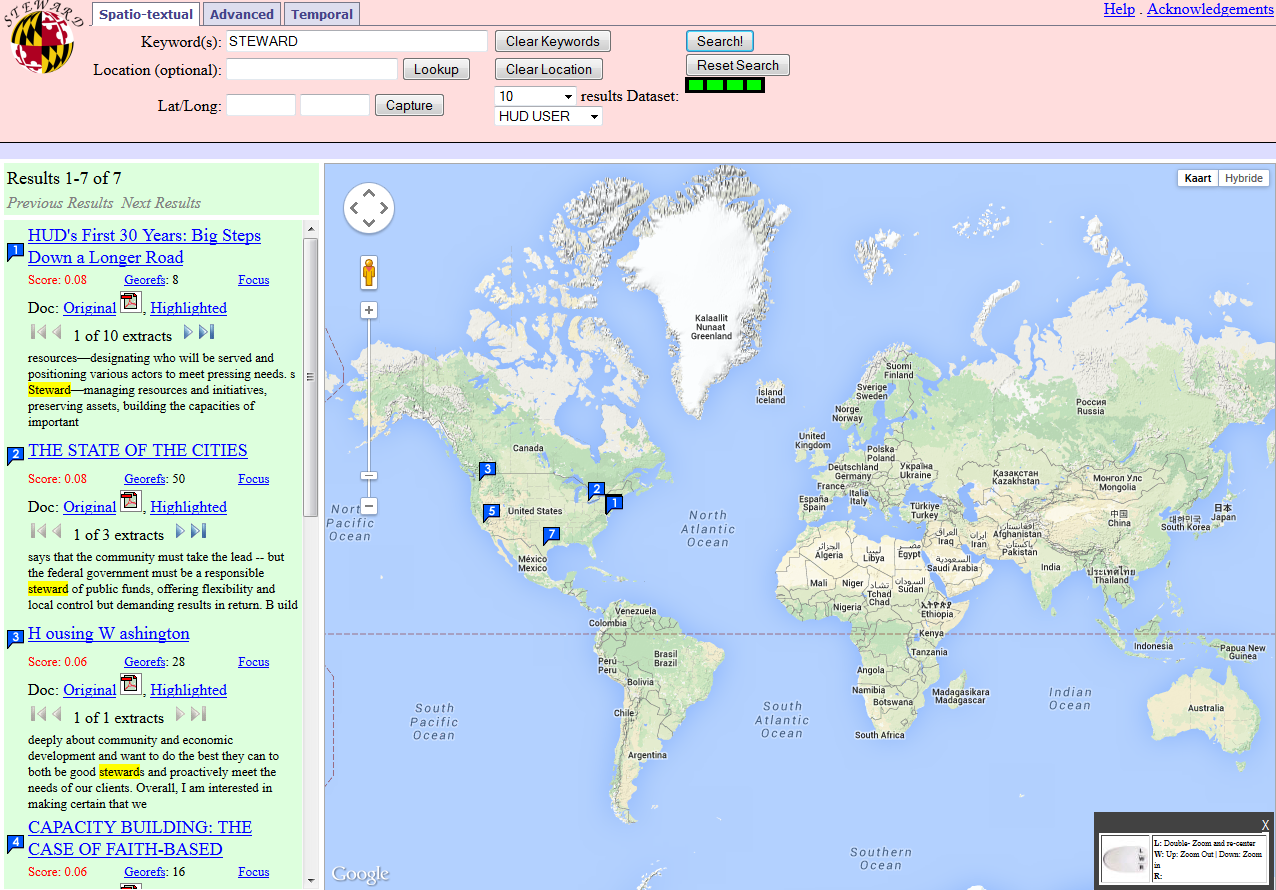
\includegraphics[scale=0.3]{./img/STEWARD.png}
			\caption{STEWARD User Interface}
		\end{figure}
		\\[0.5cm]
		Het STEWARD systeem kan gebruikt worden voor een aantal verschillende toepassingen. Bijvoorbeeld als zoekmachine voor het "hidden web"\footnote{http://en.wikipedia.org/wiki/Deep\_Web}, waar een normale zoekmachine, welke gebruik maakt van een pagerank algoritme\footnote{http://en.wikipedia.org/wiki/PageRank}, niet zal werken door het gebrek aan links naar de documenten. Ook kan er gezocht worden op nieuws, dit gaat nog wel aan de hand van een onderwerp (met eventueel een locatie). De resultaten worden vervolgens op een kaart weer gegeven zodat de gebruiker gemakkelijk kan zien wat de geografische locatie van het artikel is. Daarnaast kan het systeem gebruikt worden als een monitoring systeem voor ziektes, en het verzamelen van touristische, historische en recreationele informatie over een stad of gebied.
	\section{NewsStand: A New View on News \cite{NewsStand2008}}
		Nieuws artikelen bevatten heel veel (implicite) geografische informatie, die niet altijd duidelijk is voor de lezer. Door dit inzichtelijk te maken wordt het begrip van nieuws vergroot. NewsStand doet dit door RSS feeds \footnote{http://en.wikipedia.org/wiki/RSS} in de gaten te houden. Voor elk artikel wordt de geografische inhoud ge"extraheerd door gebruik te maken van een geotagger, de artikelen worden vervolgens geclusterd. Door in te zoomen op de kaart kunnen gebruikers nieuwsberichten vinden, afhankelijk van hoe ver een gebruiker ingezoomd is worden verschillende nieuwsberichten getoond.
		\\[0.5cm]
		In het artikel wordt besproken waarom een dergelijk systeem nuttig is, en hoe dit systeem is opgebouwd.
	\section{Reading News with Maps by Exploiting Spatial Synonyms \cite{RNwMbESS}}
		Dit artikel uit oktober 2014 is het vervolg op \textit{NewsStand: A New View on News} uit november 2008. De architectuur van NewsStand\footnote{http://newsstand.umiacs.umd.edu/web/} wordt ook in dit artikel weer besproken, net als het proces van het geotaggen en de problemen waar hier rekening mee gehouden moeten worden.
		\\[0.5cm]
		In de toekomst willen zij deze tool uitbreiden zodat er naast tekst ook geozcht kan worden op foto's, videos en audio. Ook willen ze andere soorten nieuwsbronnen gaan gebruiken zoals Twitter.
		\begin{figure}[!htb]
			\centering
			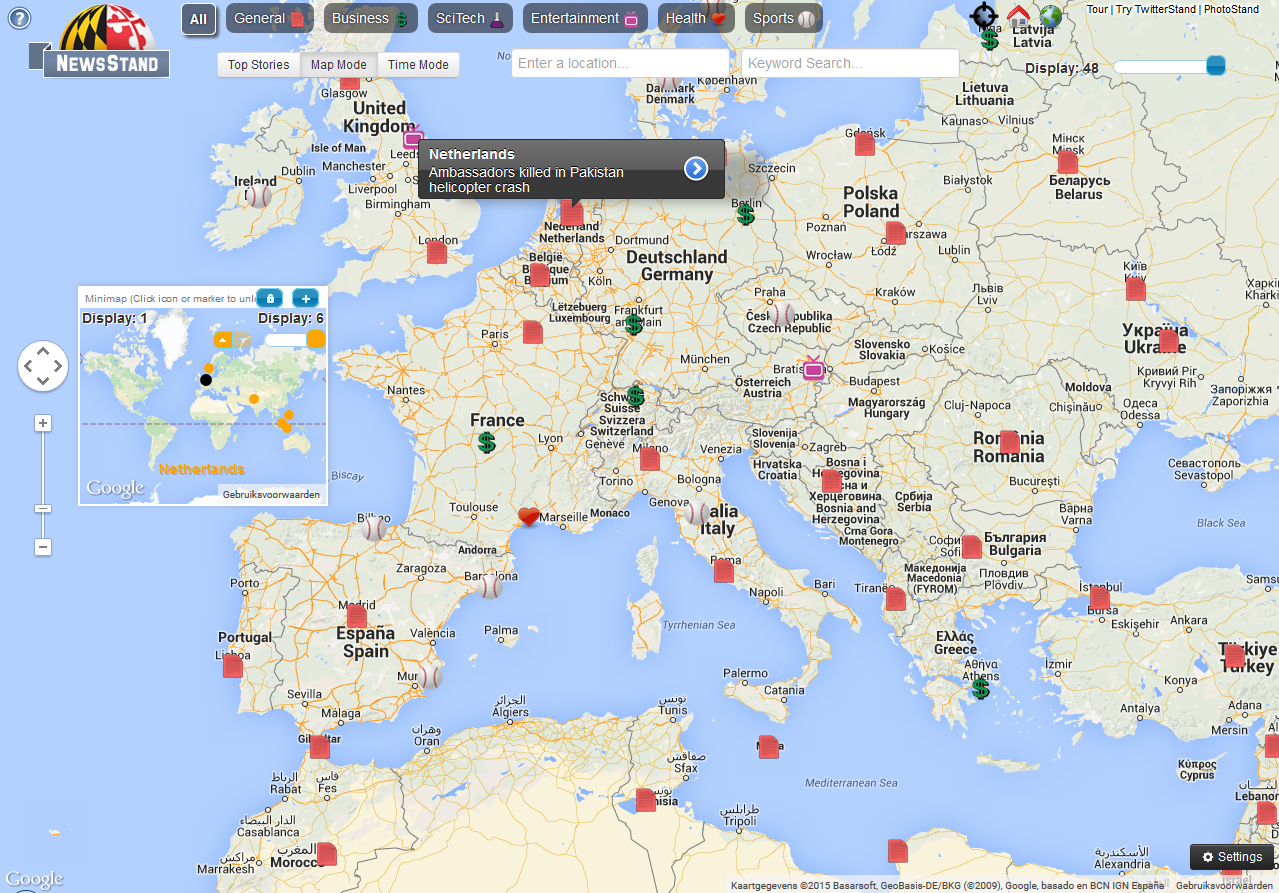
\includegraphics[scale=0.3]{./img/NewsStand.png}
			\caption{NewsStand User Interface}
		\end{figure}	
\chapter{Architectuur}
	\section{Ontwerp keuzes}
	\section{Server}
	\section{Database}
	\section{User Interface}
	
\chapter{Implementatie}
	\section{Server en database}
		\subsection{server}
		\subsection{database}
	\section{Selecteren van steden}
		\subsection{Welke steden liggen in het geselecteerde gebied?}
		Een door de gebruiker op de kaart geselecteerd gebied wordt weergegeven door de co\"ordinaten van het middelpunt (breedtegraad\footnote{http://en.wikipedia.org/wiki/Latitude} en lengtegraad\footnote{http://en.wikipedia.org/wiki/Longitude}) en de straal van de cirkel (het gebied) in kilometers.
		\\[0.5cm]
		Om te berekenen welke steden binnen dit gebied ligen moet de afstand van het middelpunt tot een stad berekend worden. Is deze afstand kleiner dan of gelijk aan de straal van het geselecteerde gebied, dan ligt de stad in het gebied.
		\\[0.5cm]
		Voor het berekenen van de afstand tussen twee punte $P_1(lat_1, lon_1)$ en $P_2(lat_2, lon_2)$ op een bol, zoals de aarde,  kan geen gebruik gemaakt worden van de stelling van Pythagoras\footnote{http://en.wikipedia.org/wiki/Pythagorean\_theorem} omdat deze stelling uit gaat van een plat vlak. Om de afstand tussen twee punten op een bol te berekenen kan gebruik gemaakt worden van bijvoorbeeld de \textit{spherical law of cosines}\footnote{http://en.wikipedia.org/wiki/Spherical\_law\_of\_cosines} of de \textit{haversine formule}\footnote{http://en.wikipedia.org/wiki/Haversine\_formula}. De \textit{haversine formule} is vooral voor kleine afstanden nauwkeuriger, met deze formule kunnen afstanden tot ongeveer 'e'en meter nauwkeurig berekend worden. Bij de \textit{spherical laq of cosines} is de maximale fout een paar meter. Om deze reden wordt de \textit{haversine formule} meer gebruikt bij navigatie, voor dit project is een fout van een paar meter echter niet belangrijk. Er is daarom gekozen voor de \textit{spherical law of cosines}.
		\\[0.5cm]
		$distance = \arccos(\sin(lat_1) \cdot \sin(lat_2) + \cos(lat_1) \cdot \cos(lat_2) \cdot(lon_1 - lon_2)) \cdot R$
		\\[0.5cm]
		Hierin zijn $(lat_1, lon_1)$ de co"ordinaten van het startpunt, in dit geval het middelpunt van het geselecteerde gebied, en $(lat_2, lon_2)$ de co"ordinaten van het tweede punt waarvoor we de afstand tot het start punt willen berekenen. Deze co"ordinaten worden door de client in graden door gestuurd en moeten eerst omgezet worden naar radialen om in deze formule gebruikt te kunnen worden. $R$ is de straal van de bol waarop beide punten liggen, in dit geval de aarde $ 	\Rightarrow R = 6371km$.
		\\[0.5cm]
		Met deze formule zou meteen een \textit{SQL\footnote{http://en.wikipedia.org/wiki/SQL} query} geconstrueerd kunnen worden.
\begin{verbatim}
SELECT
    cities.NAME, cities.LAT, cities.LON, cities.POP
FROM 
    cities 
WHERE 
    acos(sin(lat) * sin(cities.lat) + cos(lat) * cos(cities.lat) * cos(lon - cities.lon)) * 
    6371 <= radius;
\end{verbatim}
		Deze query geeft als resultaat een lijst met steden die binnen het door de gebruiker geselecteerde gebied liggen. Voor elke stad wordt de naam, populatie, breedtegraad en lengtegraad terug gegeven.
		\\[0.5cm]
		Nadeel van deze query is echter dat voor alle steden in de database berekend moet worden of de afstand tot het middelpunt van het geselecteerde gebied kleiner dan of gelijk is aan de straal van het gebied. Dit kost veel tijd, om dit te versnellen selecteren we alleen kandidaat steden waar we vervolgens de berekening op uit gaan voeren. Door de minimale en maximale breedtegraad en lengtegraad te berekenen kunnen we al een heleboel steden uitsluiten die sowieso buiten het geselecteerde gebied liggen.
		\subsubsection{Berekenen minimale en maximale breedtegraad}
		Als je van een punt $A$ naar een punt $B$ op een cirkel gaa tkun je de hoek, $r$, tussen deze twee punten berekenen. Lengtecirkels (meridianen)\footnote{http://en.wikipedia.org/wiki/Meridian\_(geography)} zijn dergelijke cirkles op aarde met een straal van $R = 6371km$. Je kan dus over een meridiaan verplaatsen, dat wil zeggen de lengtegraad blijft constant, en simpelweg $r$ aftrekken/optellen bij de breedtegraad van het middelpunte van het geselecteerde gebied om de minimale en maximale breedtegraad te krijgen.
		\\[0.5cm]
		$lat_{min} = lat - r$ \\
		$lat_{max} = lat + r$
		\\[0.5cm]
		$r$ hangt af van de afstand tussen de twee punten en de straal $R$ van de aarde. De afstand tussen de twee punten stellen we gelijk aan de maximale afstand dat een stad nog in het geselecteerde gebied ligt, dat is de straal van het gebied.
		\\[0.5cm]
		$r = max. distance / R = radius / R$
		\subsubsection{Berekenen minimale en maximale lengtegraad (methode 1)}
		\subsubsection{Berekenen minimale en maximale lengtegraad (methode 2)}
		De methode omschreven in de vorige sectie om de minimale en maximale lengtegraad te berekenen werkt dus niet goed. Dit is te zien in figuur \ref{fig:tangentpoints}, de punten op de cirkel met de minimale en maximale lengtegraad $T_1$ en $T_2$ liggen niet op de zelfde breedtecirkel\footnote{http://en.wikipedia.org/wiki/Circle\_of\_latitude} als $M$, het middelpunt van het geselecteerde gebied maar dichter bij de pool.
		\begin{figure}[!htb]
			\centering
			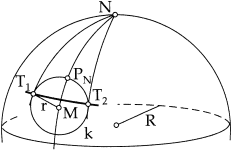
\includegraphics[scale=1.0]{./img/TangentPoints.png}
			\caption{Tangent meridians to the query circle}
			\label{fig:tangentpoints}
		\end{figure}
		\newpage
		In plaats daar van moeten de volgende formules gebruikt worden
		\\[0.5cm]
		$lat_T = \arcsin(\sin(lat)/\cos(r))$\\
		$lon_{min} = lon_{T_1} = lon - \Delta lon$\\
		$lon_{max} = lon_{T_2} = lon + \Delta lon$
		\\[0.5cm]
		$\Delta lon = \arccos((\cos(r) - \sin(lat_T) \cdot \sin(lat)) / (\cos(lat_T) \cdot \cos(lat)))$ \\
		$= \arcsin(\sin(r) / cos(lat))$
		\subsubsection{SQL query}
		Aan dde hand van de hierboven berekende minimale en maximale breedtegraad en lengtegraad kunnen we nu een SQL query maken die de berekening, de spherical law of cosines, alleen hoeft uit te voeren op een veel kleiner aantal kandidaat plaatsen.
\begin{verbatim}
SELECT
    cities.NAME, cities.LAT, cities.LON, cities.POP
FROM 
    cities 
WHERE 
        (cities.LAT >= lat_min AND cities.LAT <= lat_max) 
    AND 
        (cities.LON >= lon_min AND cities.LON <= lon_max) 
GROUP BY
    cities.NAME
HAVING
    acos(sin(lat) * sin(cities.LAT) + cos(lat) * cos(cities.LAT) * 
         cos(cities.LON - (lon))) <= radius;
\end{verbatim}
Deze query selecteerd de naam, breedtegraad, lengtegraad en populatie voor elke stad die binnen het geselecteerde gebied valt. Eerst worden alle steden geselecteerd waarvoor de breedtegraad en de lengtegraad binnen de minimale en maximale waardes vallen. Vervolgens wordt voor elk van deze kandidaat plaatsen uitgerekend of deze ook echt binnen het geselecteerde gebied liggen. De query is vervolgens aangepast om ook de landen waarin de steden liggen te selecteren. Dit is nodig omdat sommige steden in meerdere landen voorkomen. Doe je dit niet kan het voorkomen dat je nieuws uit een heel ander wereld deel krijgt dan het gebied wat de gebruiker geselecteerd heeft.
\begin{verbatim}
SELECT
    cities.NAME, cities.LAT, cities.LON, cities.POP, countries.NAME
FROM 
    cities, countries 
WHERE
        cities.COUNTRY_CODE = countries.CODE 
    AND
        (cities.LAT >= lat_min AND cities.LAT <= lat_max) 
    AND 
        (cities.LON >= lon_min AND cities.LON <= lon_max) 
GROUP BY
    cities.NAME
HAVING
    acos(sin(lat) * sin(cities.LAT) + cos(lat) * cos(cities.LAT) * 
         cos(cities.LON - (lon))) <= radius;
\end{verbatim}
% CONTROLEREN!
Omdat een deel van de steden in de database een populatie van $0$ heeft (ongeveer $30000$ van de $ 140000$ steden), en het algoritme voor de gebiedsrepresentatie de grootste stad in een gebied moet vinden selecteren we alleen de steden waarvan de populatie \textbf{niet} $0$ is.
\begin{verbatim}
SELECT
    cities.NAME, cities.LAT, cities.LON, cities.POP, countries.NAME
FROM 
    cities, countries 
WHERE
        cities.COUNTRY_CODE = countries.CODE 
    AND
        (cities.LAT >= lat_min AND cities.LAT <= lat_max) 
    AND 
        (cities.LON >= lon_min AND cities.LON <= lon_max)
    AND
        cities.pop != 0
GROUP BY
    cities.NAME
HAVING
    acos(sin(lat) * sin(cities.LAT) + cos(lat) * cos(cities.LAT) * 
         cos(cities.LON - (lon))) <= radius;
\end{verbatim}
	\section{Gebieds representatie}
		Bij het geselecteerde gebied worden vaak honderd of meer, en bij een groot gebied duizenden, steden gevonden die in dit gebied liggen. Om voor elke stad naar nieuws te zoeken levert evenveel zoekopdrachten als steden op. Dit gaat erg veel tijd in beslag nemen, ongeveer $300ms$ per zoekopdracht, en levert te veel nieuws op. Een dergelijke hoeveelheid nieuws, in de orde van duidezenden artikelen, is voor de gebruker niet te verwerken en draagt niet bij aan een beter begrip van het nieuws en wat er in het gebied gaande is.
		\\[0.5cm]
		Een gebied moet dus door een kleiner aantal steden gerepresenteerd worden zodat het aantal zoekopdrachten beperkt blijft en de gebruiker de hoeveelheid nieuws goed kan verwerken. Hiervoor zijn verschillende optie die hieronder besproken zullen worden.
		
		\subsubsection{Aantal steden om een gebied te representeren}
			Het aantal steden om een gebied te representeren is bepaald aan de hand van een gebruikersonderzoek. De opzet en resultaten van dit onderzoek worden bepsroken in sectie \ref{sec:numcities}.
			\\[0.5cm]
			Daarnaast wordt er rekening mee gehouden dat er voor een kleiner gebied minder steden nodig zijn om dit gebied te respresenteren dan bij een groter gebied.
		\subsection{Algoritme 1}
			Dit algoritme reduceerd een lijst steden tot een maximum aantal zodat een gebied goed gerepresenteerd wordt. Dit gaat op de volgende manier:
			\begin{algorithm}
				\caption{Algortime 1 voor gebiedsrepresentatie}
				\mbox{Split():}\\[0.5cm]
				\KwIn{list of cities}
				\KwResult{Reduced list of cities representing the area}
				\mbox{}\\
				\While{number of result $<$ number of cities to represent the area}{
						find biggest city;\\
						add to result;\\
						\mbox{}\\
						\ForEach{city}{
							calculate bearing;\\
							add to corresponding sublist (nw/ne/se/sw);
							}
							\mbox{}\\
						\ForEach{sublist (nw/ne/se/sw)}{
							\eIf{number of cities $<= 5$}{
								find biggest city;\\
								add to result;
								}{
								Split(sublist);\\
								add to result;
								}
							}
					}
			\end{algorithm}\\[0.5cm]
			Dit recursieve algoritme heeft als input een lijst met steden, dit zijn in eerste instantie alle steden die in het door de gebruiker op de kaart geselecteerde gebied liggen. De grootste stad in dit gebied wordt gezocht ena an het eind resultaat toegevoegd. Vervolgens wordt het gebied in vier delen opgedeeld: Noord-Oost, Zuid-Oost, Zuid-West en Noord-West, zie figuur \ref{fig:bearing}. Om deze opdeling te maken wordt voor elke stad de richting, ten opzichte van de gootste stad, berekend (algoritme \ref{alg:bearing}) en aan het juiste deel gebied toegevoegd.
			\begin{figure}[!htb]
				\centering
				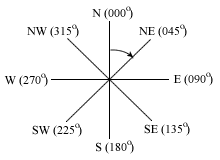
\includegraphics[scale=1.0]{./img/bearings.png}
				\caption{Deelgebieden en hun richting}
				\label{fig:bearing}
			\end{figure}
			\begin{algorithm}
				\caption{Berekenen van de richting}
				\label{alg:bearing}
				\mbox{GetBearing():}\\[0.5cm]
				\KwIn{$(lat_1, lon_1)$, $(lat_2, lon_2)$}
				\KwOut{Bearing in degrees}
				\mbox{}\\
				convert $(lat_1, lon_1)$, $(lat_2, lon_2)$ to radians;\\
				\mbox{}\\
				$\Delta lon = lon_2 - lon_1;$\\
				\mbox{}\\
				$x = \sin(\Delta lon) \cdot \cos(lat_2);$\\
				$y = \cos(lat_1) \cdot \sin(lat_2) - (\sin(lat_1) \cdot \cos(lat_2) \cdot \cos(\Delta lon));$\\
				\mbox{}\\
				$bearing = \arctan(x/y);$\\
				\mbox{}\\
				convert bearing to degrees;\\
				\mbox{}\\
				$bearing = (bearing + 360.0) / 360.0;$\\
			\end{algorithm}
			Als het aantal steden in een deel gebied kleiner dan of gelijk is aan $5$ wordt de grootste stad in het deelgebied gezocht en aan het eind resultaat toegevoegd. Is het aantal steden echter groter dan wordt het hier boven beschreven proces herhaald voor het deelgebied. \\[0.5cm]
			Aan het einde geeft dit algoritme een lijst van steden die het gebied representeren. Als deze lijst nog steeds meer steden bevat dan het maximale aantal steden om een gebied te representeren wordt dit proces herhaald.
		\subsection{Algoritme 2}
			Een andere mogelijkehid om een aantal steden die een gebied vertegenwoordigen te selecteren is weer de gootste stad kiezen maar nu het gebied in twee delen splitsen in plaats van vier zoals bij het hier boven beschreven algortime.
			\begin{algorithm}
				\caption{Algoritme 2 voor gebiedsrepresentatie}
				\mbox{Split():}\\[0.5cm]
				\KwIn{list of cities}
				\KwResult{Reduced list of cities representing the area}
				\mbox{}\\
				\While{number of result $<$ number of cities to represent the area}{
					find biggest city;\\
					add to result;\\
					\mbox{}\\
					\ForEach{city}{
						calculate bearing;\\
						add to corresponding sublist (nw/ne/se/sw);
					}
					\mbox{}\\
					\ForEach{sublist (nw/ne/se/sw)}{
						\eIf{number of cities $<= 5$}{
							find biggest city;\\
							add to result;
						}{
							Split(sublist);\\
							add to result;
						}
					}
				}
			\end{algorithm}\\[0.5cm]
			Het algoritme kiest de grootste stad in het gebied, vevolgens wordt er gekeken welke steden ten noorde liggen en welke steden ten zuide. Voor elk van deze twee deel gebieden wordt weer de grootste stad gezocht, en daarna worden deze deel gebieden opnieuw gesplitst maar nu in oost en west.\\[0.5cm]
			Voor elk deel gebied wordt dus telkens de grootste staad gezocht en deze wordt aan het eind resultaat toegevoegd. het splitsen van een deelgebied gaat om en om: eerst wordt het gebied in noord en zuid gesplitst, dan wordt elk deel gebied in oost en west gesplitst. Nu hebben we vier deelgebieden die allen weer in noord en zuid worden verdeeld etc.
		\subsection{Andere opties}
			Naast deze twee algoritmes zijn er nog enkele andere mogelijkheden om steden te kiezen om een gebied te representeren. Deze werken echter minder goed dan de hier boven beschreven algoritmes.
			\subsubsection{Grootste steden}
				Een mogelijkheid is om alleen de grootste steden in een gebied te selecteren. Voordeel is dat dit een snel en eenvoudig proces is, nadeel is echter dat de verdeling van de grote steden over het gebied (vaak) niet uniform is met als gevolg dat de geselecteerde steden geen goede representatie van het gebied geven.
				%IMAGE
				Een ander probleem bij het selecteren van alleen de grootste steden is dat grote steden, zoals bijvoorbeeld Londen, in meerdere delen in de database staan. Als je nu de grootste steden kiest worden vaak alle drie de delen gekozen met als gevolg dat er clusters ontstaan en er minder steden in de rest van het gebied gekozen kunnen worden.
			\subsubsection{Hoofdsteden}
				In het geval van een selectie van meerdere landen is het een mogelijkheid om alleen de hoofdsteden te gebruiken voor de representatie eventueel aangevuld met de grootste steden in het gebied om voldoende steden te krijgen. Dit is eigenlijk alleen een goede optie als er precies even veel landen als benodigde steden in het gebied liggen. Liggen er minder landen in het gebied, en wordt er aangevuld met de grootste steden, loop je hoogst waarschijnlijk tegen het zelfde probleem aan als wanneer je alleen maar voor de grootste steden kiest. Daarbij komt dat het resultaat vaak nagenoeg gelijk zal zijn omdat hoofdsteden vaak bij de grotere steden horen. 
			\subsubsection{Willekeurig}
				Uit de lijst met steden die in het gebied liggen kunnen willekeurig een aantal steden gekozen worden welke dit gebied representeren. Omdat het hier mogelijk is dat alleen (of grotendeels) kleine/de kleinste steden gekozen worden is dit een minder geschikte mogelijkheid.  Ook is het, net als bij boven genomende methodes, mogelijk dat de gekozen steden niet verspreid liggen maar zich concentreren in een klein deel van het gebied. Ander groot probleem is dat elke keer dat de gebruiker een gebied selecteert een andere lijst aan steden terug gegeven wordt, hierdoor zullen er elke keer andere nieuws artikelen gezocht worden. Het wordt hierdoor moeilijker (onmogelijk) om een artikel opnieuw op te zoeken met de tool.
\chapter{Experimenten}
	Om te weten of de ontwikkelde applicatie echt een toegevoegde waarde is moeten er een gebruikers onderzoek uitgevoerd worden. Daarnaast is er een onderzoek nodig om een te bepalen hoeveel steden er nodig zijn om een gebied te representeren, en om een keuze te maken uit de twee voorgestelde algoritmes om deze steden te kiezen.
	\section{Gebiedsrepresentatie}
	\label{sec:numcities}
		Dit onderzoek is gedaan om te bepalen hoeveel steden er nodig zijn om een gebied goed te representeren. Ook wordt er gekeken welke van de twee voorgestelde algoritmes het beste is om de steden te selecteren die het gebied gaan representeren.
		\subsection{Opzet}
			Voor dit experiment is een enqu\^ete gemaakt waarin de gebruiker een afbeelding van een geselecteerd gebied te zien krijgt. Een voorbeeld hiervan wordt gegeven in afbeelding \ref{fig:area_rep}.
			\begin{figure}[!htb]
				\centering
				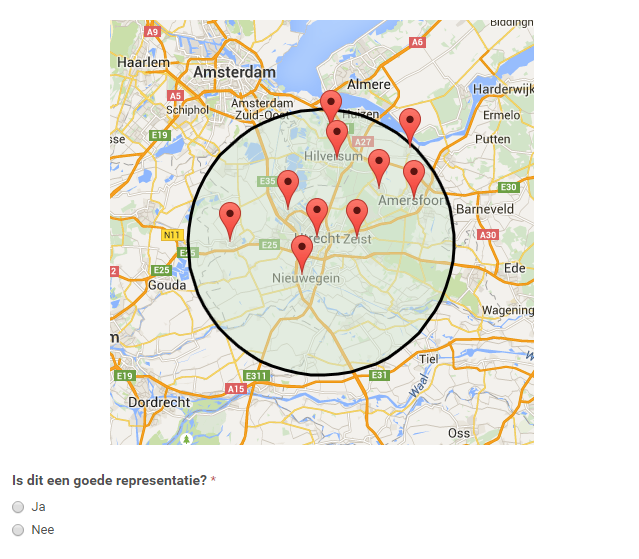
\includegraphics[scale=0.8]{./img/area_rep.png}
				\caption{Voorbeeld vraag gebiedsrepresentatie}
				\label{fig:area_rep}
			\end{figure}
			Bij elke afbeelding krijgt de gebruiker de vraag of dit een goede representatie is van het geselecteerde gebied. Dit is een meerkeuze vraag met als mogelijke antwoorden \textit{ja} en \textit{nee}. Wanneer de gebruiker \textit{nee} kiest krijgt hij of zij een afbeelding van het zelfde gebied te zien maar met meer steden. Er zijn afbeeldingen met tien, vijftien en twintig steden. Zodra er ja gekozen wordt krijgt de gebruiker een vervolg vraag om te bepalen welke van de twee voorgestelde algoritmes beter is. Hiervoor krijgt hij of zij twee afbeeldingen van het zelfde gebied te zien, met het door hem of haar gekozen aantal steden. Een van de afbeeldingen is met algoritme 1 gemaakt terwijl de andere algoritme 2 gebruikt. De vraag is nu welke van de twee representaties beter is, met als mogelijke antwoorden optie 1 of optie 2. Afbeelding \ref{fig:algo} is hier een voorbeeld van. In totaal zijn er voor vier gebebied vragen, dit zijn gebieden met een straal van $25km$, $100km$, $500km$ en $1000km$.
			\\[0.5cm]
			Deze enqu\^ete is in met Google Docs\footnote{http://docs.google.com/} gemaakt en de resultaten worden in een \textit{.xls} bestand opgeslagen.
			\begin{figure}[!htb]
				\centering
				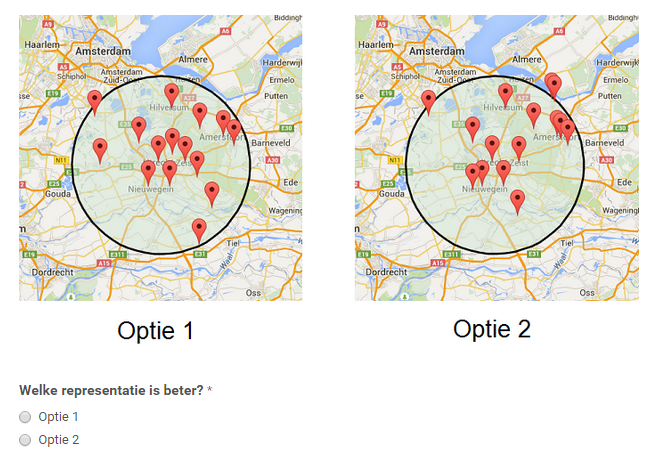
\includegraphics[scale=0.8]{./img/algo.png}
				\caption{Voorbeeld vraag gebiedsrepresentatie}
				\label{fig:algo}
			\end{figure}	
		\newpage		
		\subsection{Resultaten}
			De resultaten zoals deze in het \textit{.xls} bestand opgeslagen zijn zijn te vinden in bijlage \ref{app:results_rep}. Hier onder worden de resultaten per gebied besproken. De enqu\^ete is door twintig mensen ingevuld met een leeftijd van 15 tot en met 80 jaar. Er zitten ongeveer evenveel mannen als vrouwen in deze groep met allemaal een verschillend opleidings niveau. Dit is gedaan om een zo goed mogelijk beeld te krijgen van de hoeveelheid steden die nodig is en wat het beste algoritme is.
			\subsubsection{Gebied 1 - straal 25km}
				In tabel \ref{tab:res25} zijn de resultaten te zien voor een gebied met een straal van $25km$. Aan de hand van deze resultaten kunnen we het gemiddelde aantal steden berekenen dat nodig is om dit gebied te representeren: $(10 * 10 + 9 * 15 + 2 * 20) / 21 \approx 13.09$ steden. Verder is te zien dat $(19 / 21)  * 100\%\approx 90.48\%$ van de respondenten de representatie gegeven door algoritme 1 beter vindt, $(2 / 21) * 100\% \approx 9.52\%$ kiest voor algoritme 2.
				\begin{table}[!htb]
					\centering
					\begin{tabular}{| c | c | c | c | c |}
						\hline	
						\textbf{Kandidaat} & \textbf{10 steden} & \textbf{15 steden} & \textbf{20 steden} & \textbf{Algoritme} \\ \hline
						1 & \ding{56} & \ding{52} &  & 1 \\ \hline
						2 & \ding{56} & \ding{52} &  & 1 \\ \hline
						3 & \ding{56} & \ding{52} &  & 1 \\ \hline
						4 & \ding{52} &  &  & 1 \\ \hline
						5 & \ding{52} &  &  & 1 \\ \hline
						6 & \ding{56} & \ding{52} &  & 1 \\ \hline
						7 & \ding{56} & \ding{52} &  & 1 \\ \hline
						8 & \ding{56} & \ding{52} &  & 1 \\ \hline
						9 & \ding{52} &  &  & 1 \\ \hline
						10 & \ding{52} &  &  & 1 \\ \hline
						11 & \ding{52} &  &  & 1 \\ \hline
						12 & \ding{56} & \ding{56} & \ding{52} & 2 \\ \hline
						13 & \ding{52} &  &  & 1 \\ \hline
						14 & \ding{52} &  &  & 1 \\ \hline
						15 & \ding{52} &  &  & 1 \\ \hline
						16 & \ding{56} & \ding{52} &  & 1 \\ \hline
						17 & \ding{52} &  &  & 1 \\ \hline
						18 & \ding{52} &  &  & 1 \\ \hline					
						19 & \ding{56} & \ding{52} &  & 2 \\ \hline
						20 & \ding{56} & \ding{52} &  & 1 \\ \hline
						21 & \ding{56} & \ding{56} & \ding{52} & 1 \\ \hline
					\end{tabular}
					\caption{Resultaten voor een gebied met straal 25km}
					\label{tab:res25}
				\end{table}
			\subsubsection{Gebied 2 - straal 100km}
				In tabel \ref{tab:res100} zijn de resultaten te zien voor een gebied met een straal van $100km$. Aan de hand van deze resultaten kunnen weer het gemiddelde aantal steden berekenen dat nodig is om dit gebied te representeren: $(7 * 10 + 8 * 15 + 3 * 20) / 19 \approx 13.16$ steden. Verder is te zien dat $(18 / 21)  * 100\%\approx 85.71\%$ van de respondenten de representatie gegeven door algoritme 1 beter vindt, $(3 / 21) * 100\% \approx 14.29\%$ kiest voor algoritme 2. Er is hier bij het berekenen van het gemiddelde aantal steden dat nodig is voor de weergave van dit gebied gedeeld door $19$ omdat twee respondenten geen van de drie representaties goed vonden. Omdat er ook als er op alle drie de vragen nee geantwoord een keuze gemaakt moet worden tussen de twee algoritmes is hier wel door $21$ gedeeld.
				\begin{table}
					\centering
					\begin{tabular}{| c | c | c | c | c |}
						\hline	
						\textbf{Kandidaat} & \textbf{10 steden} & \textbf{15 steden} & \textbf{20 steden} & \textbf{Algoritme} \\ \hline
						1 & \ding{56} & \ding{52} &  & 1 \\ \hline
						2 & \ding{56} & \ding{52} &  & 1 \\ \hline
						3 & \ding{56} & \ding{56} & \ding{52} & 1 \\ \hline
						4 & \ding{56} & \ding{52} &  & 1 \\ \hline
						5 & \ding{56} & \ding{56} & \ding{52} & 1 \\ \hline
						6 & \ding{52} &  &  & 1 \\ \hline
						7 & \ding{56} & \ding{52} &  & 2 \\ \hline
						8 & \ding{52} &  &  & 2 \\ \hline
						9 & \ding{56} & \ding{56} & \ding{56} & 1 \\ \hline
						10 & \ding{52} &  &  & 1 \\ \hline
						11 & \ding{52} &  &  & 1 \\ \hline
						12 & \ding{56} & \ding{56} & \ding{52} & 1 \\ \hline
						13 & \ding{52} &  &  & 1 \\ \hline
						14 & \ding{56} & \ding{56} & \ding{56} & 1 \\ \hline
						15 & \ding{56} & \ding{52} &  & 1 \\ \hline
						16 & \ding{52} &  &  & 1 \\ \hline
						17 & \ding{56} & \ding{56} & & 1 \\ \hline
						18 & \ding{52} &  &  & 2 \\ \hline					
						19 & \ding{56} & \ding{52} &  & 1 \\ \hline
						20 & \ding{56} & \ding{52} &  & 1 \\ \hline
						21 & \ding{56} & \ding{52} &  & 1 \\ \hline
					\end{tabular}
					\caption{Resultaten voor een gebied met straal 100km}
					\label{tab:res100}
				\end{table}
			\subsubsection{Gebied 3 - straal 500km}
				In tabel \ref{tab:res500} zijn de resultaten te zien voor een gebied met een straal van $500km$. Ook nu weer kunnen we aan an de hand van deze resultaten het gemiddelde aantal steden berekenen dat nodig is om dit gebied te representeren: $(9 * 10 + 9 * 15 + 3 * 20) / 21 \approx 13.57$ steden. Verder is te zien dat $(20 / 21)  * 100\%\approx 95.24\%$ van de respondenten de representatie gegeven door algoritme 1 beter vindt, $(1 / 21) * 100\% \approx 4.76\%$ kiest voor algoritme 2.
				\begin{table}
					\centering
					\begin{tabular}{| c | c | c | c | c |}
						\hline	
						\textbf{Kandidaat} & \textbf{10 steden} & \textbf{15 steden} & \textbf{20 steden} & \textbf{Algoritme} \\ \hline
						1 & \ding{56} & \ding{52} &  & 1 \\ \hline
						2 & \ding{56} & \ding{52} &  & 1 \\ \hline
						3 & \ding{56} & \ding{56} & \ding{52} & 1 \\ \hline
						4 & \ding{56} & \ding{52} &  & 1 \\ \hline
						5 & \ding{56} & \ding{56} & \ding{52} & 1 \\ \hline
						6 & \ding{52} &  &  & 1 \\ \hline
						7 & \ding{56} & \ding{52} &  & 1 \\ \hline
						8 & \ding{52} &  &  & 1 \\ \hline
						9 & \ding{52} &  &  & 1 \\ \hline
						10 & \ding{52} &  &  & 1 \\ \hline
						11 & \ding{56} & \ding{52} &  & 1 \\ \hline
						12 & \ding{56} & \ding{56} & \ding{52} & 1 \\ \hline
						13 & \ding{56} & \ding{52} &  & 1 \\ \hline
						14 & \ding{52} &  &  & 1 \\ \hline
						15 & \ding{56} & \ding{52} &  & 2 \\ \hline
						16 & \ding{56} & \ding{52} &  & 1 \\ \hline
						17 & \ding{52} &  &  & 1 \\ \hline
						18 & \ding{56} & \ding{52} &  & 1 \\ \hline					
						19 & \ding{52} &  &  & 1 \\ \hline
						20 & \ding{52} &  &  & 1 \\ \hline
						21 & \ding{52} &  &  & 1 \\ \hline
					\end{tabular}
					\caption{Resultaten voor een gebied met straal 500km}
					\label{tab:res500}
				\end{table}
			\subsubsection{Gebied 4 - straal 1000km}
				De resultaten voor een gebied met een straal van $1000km$ zijn te zien in tabel \ref{tab:res1000}. Aan de hand van deze resultaten kunnen we weer het gemiddelde aantal steden berekenen dat nodig is om dit gebied te representeren: $(12 * 10 + 2 * 15 + 7 * 20) / 21 \approx 13.81$ steden. Verder is te zien dat $(19 / 21)  * 100\%\approx 95.24\%$ van de respondenten de representatie gegeven door algoritme 1 beter vindt, $(1 / 21) * 100\% \approx 4.76\%$ kiest voor algoritme 2.
			\begin{table}
				\centering
				\begin{tabular}{| c | c | c | c | c |}
					\hline	
					\textbf{Kandidaat} & \textbf{10 steden} & \textbf{15 steden} & \textbf{20 steden} & \textbf{Algoritme} \\ \hline
					1 & \ding{56} & \ding{56} & \ding{52} & 1 \\ \hline
					2 & \ding{56} & \ding{52} &  & 1 \\ \hline
					3 & \ding{56} & \ding{56} & \ding{52} & 2 \\ \hline
					4 & \ding{56} & \ding{52} &  & 1 \\ \hline
					5 & \ding{56} & \ding{56} & \ding{52} & 1 \\ \hline
					6 & \ding{52} &  &  & 1 \\ \hline
					7 & \ding{52} &  &  & 1 \\ \hline
					8 & \ding{52} &  &  & 1 \\ \hline
					9 & \ding{52} &  &  & 1 \\ \hline
					10 & \ding{52} &  &  & 1 \\ \hline
					11 & \ding{52} &  &  & 1 \\ \hline
					12 & \ding{56} & \ding{56} & \ding{52} & 1 \\ \hline
					13 & \ding{52} &  &  & 1 \\ \hline
					14 & \ding{52} &  &  & 1 \\ \hline
					15 & \ding{52} &  &  & 1 \\ \hline
					16 & \ding{56} & \ding{56} & \ding{52} & 1 \\ \hline
					17 & \ding{52} &  &  & 1 \\ \hline
					18 & \ding{56} & \ding{56} & \ding{52} & 1 \\ \hline					
					19 & \ding{52} &  &  & 1 \\ \hline
					20 & \ding{52} &  &  & 1 \\ \hline
					21 & \ding{56} & \ding{56} & \ding{52} & 1 \\ \hline
				\end{tabular}
				\caption{Resultaten voor een gebied met straal 1000km}
				\label{tab:res1000}
			\end{table}
	\section{Accuraatheid}
		\subsection{Geotagging nieuws}
		\subsection{Locatie selectie}
	\section{User Acceptance Test}
	
\chapter{Conclusie}
	\section{Conclusie}
	\section{Toekomstig onderzoek}
	
\begin{thebibliography}{9}
	\bibitem{NewsStand2008} 
	Benjamin E. Teiler, Micheal D. Lieberman, Daniele Panozzo, Jagan Sankaranarayanan, Hanan Samet and Jon Sperling.
	\textit{NewsStand: A New View on News}. 
	In Proceedings of the 16th ACM SIGSPATIAL International Conference on Advances in Geographic Information Systems (ACM GIS 2008), IRVINE, CA, November 2008
	
	\bibitem{STEWARD}
	Micheal D. Lieberman, Hanan Samet, Jagan Sankaranarayanan and Jon Sperling.
	\textit{STEWARD: Architecture of a Spatio-Textual Search Engine}
	15th ACM GIS, Seattle, WA, November 2007
	
	\bibitem{RNwMbESS}
	Hanan Samet, Jagan Sankaranarayanan, Micheal D. Lieberman, Marco D. Adelfio, Brendan C. Fruin, Jack M. Lotkowski, Daniele Panozzo, Jon Sperling and Bejamin E. Teiler.
	\textit{Reading News with Maps by Exploiting Spatial Sysnonyms}
	Communications of the ACM, Okotber 2014
\end{thebibliography}
\newpage
\appendix
\chapter{Resultaten onderzoek gebiedsrepresentatie}
\label{app:results_rep}
RESULTATEN GEBIEDS REPRESENTATIE
\end{document}